Class notes for 1-26-16

\subsection*{Null Job Topics}
Null Job: something computers do when there is nothing else to do. 
\begin{itemize}
\item{DFT $\rightarrow$ DTFT $\rightarrow$ FT $\rightarrow$ LT $\rightarrow$ ZT 
$\rightarrow$ DTFT and DFT}
\item{BW of a pole}
\item{Decay Time of a Pole}
\item{Partial Fraction Expansion (PFE)}
\item{Laplace transform}
\end{itemize}

How do you define stability? If the poles are inside the unit circle, it's
stable.
If it's on the unit circle, it is marginally stable. 

\subsection*{Unilateral transform}

\subsection*{Diff Thm transform}

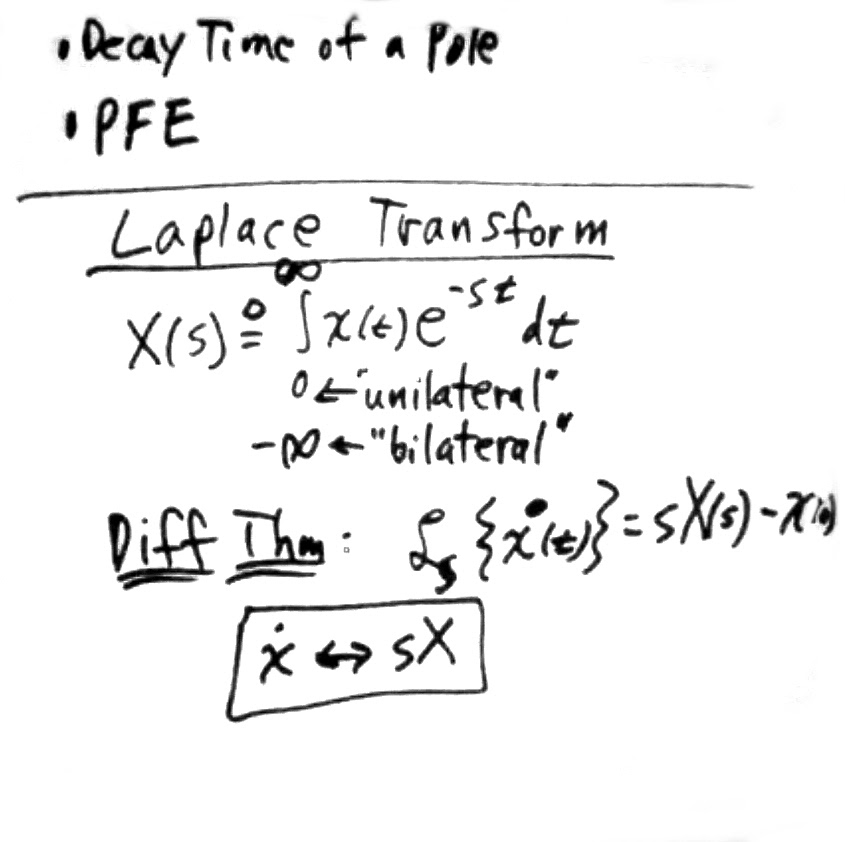
\includegraphics[scale=0.3]{photos/jan26/11a}

This is the counterpart to shift theorem for DFTs. 

\paulhint{Started new recording on a new SD card. woops}

%\paulhint{Little graphic about a "slice", taken at 15:16, 11b}

\subsection*{History of Harmonic Analysis}
History of Harmonic Analysis: darigol (sp?), which goes back to 
Daniel Bernouli. Began summing sinusoidal components "pure vibration". 
A bit later, (name?) began coming up with wave equation for vibrating string. 

You CAN make a progressive wave out of standing waves. 

First thereom: jean baptiste fourier. Had the right idea, but 
didn't have the right proof. He was working on heat diffusion. 

\subsection*{3db Bandwidth of a Pole}
Best to look at the s-plane:

Pole at P. To get the frequency response, plug in $j\omega$ into the transfer
function. 

For s-plane, left is stable and right is unstable. 

\paulhint{TODO: look at s-plane from MDFT book}

What do we need to measure 3db bandwidth? We need magnitude response 
(amplitude response). 
Let's let $P = \sigma_p$

Max is at $\omega = 0$;

%\paulhint{Picture taken at 15:30. he's still drawing though. mark at 1. 11c}

What kind of filter is this? We drew it. 

%\paulhint{Picture taken at 15:33. Note the diagram. 11b}
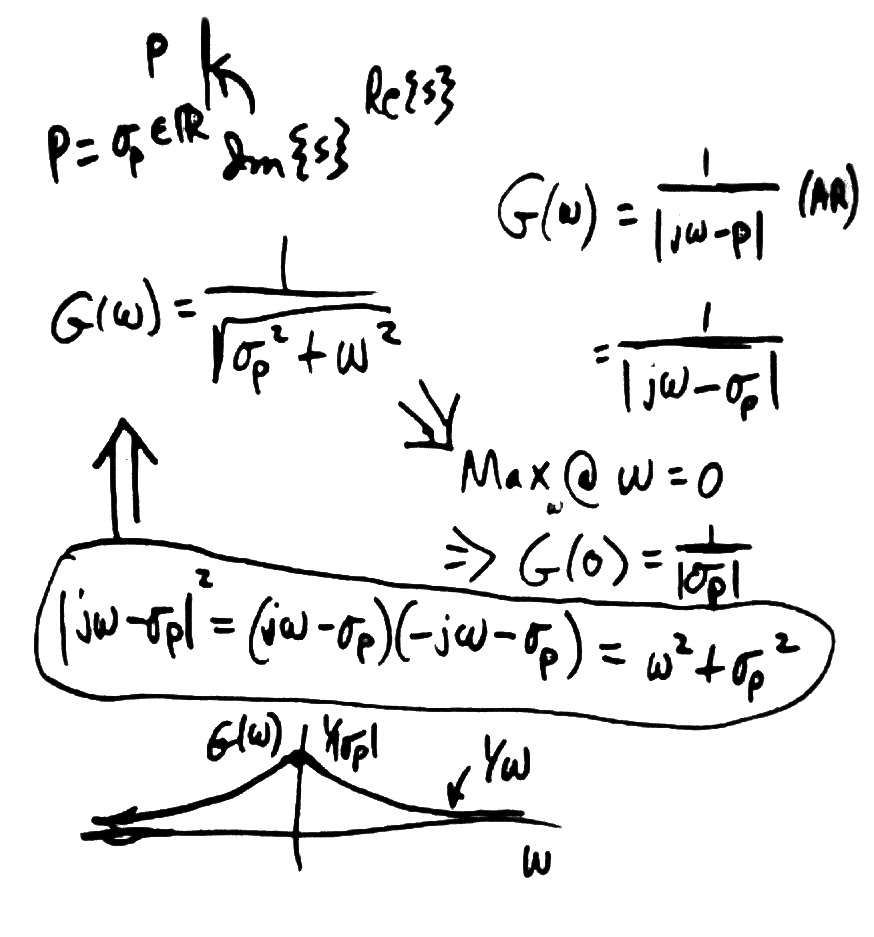
\includegraphics[scale=0.3]{photos/jan26/11b}

Q is center frequency divided by bandwidth. 

$Q = fc/B = 0$

\josquote{When it comes to filters, keep them real. Keep them rational}

\subsection*{Bandpass vs Lowpass}

\subsection*{What does constant Q mean?}

%\paulhint{See picture taken at 15:40. 11c}
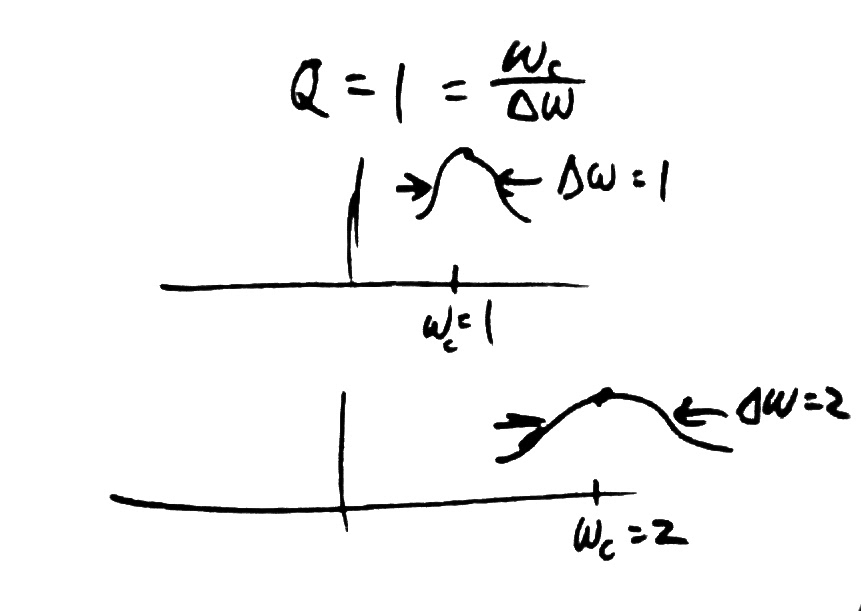
\includegraphics[scale=0.3]{photos/jan26/11c}

\subsection*{Constant Q filter bank}

%\paulhint{See picture taken at 15:41. 11d}
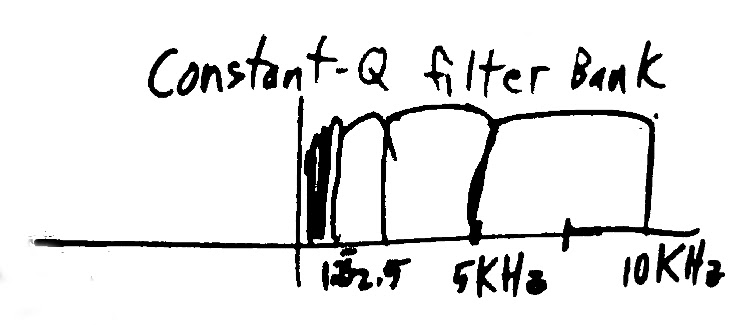
\includegraphics[scale=0.3]{photos/jan26/11d}


\subsection*{Butterworth lowpass}

%\paulhint{See picture taken at 15:43. 11e}
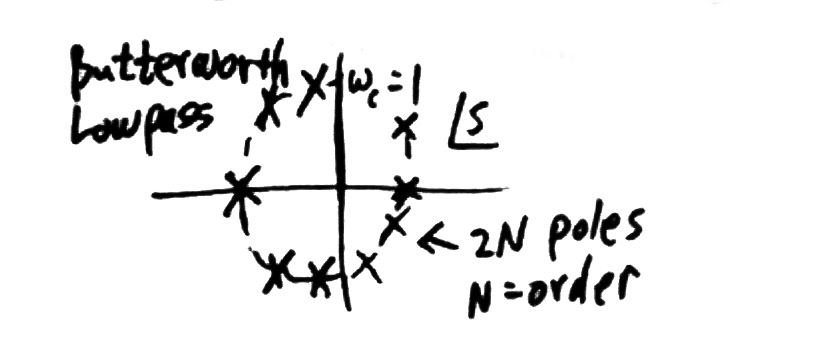
\includegraphics[scale=0.3]{photos/jan26/11e}

\paulhint{What does LHP mean?}

\subsection*{1 Pole Butterworth}

%\paulhint{See picture taken at 15:46. 11f.jpg}
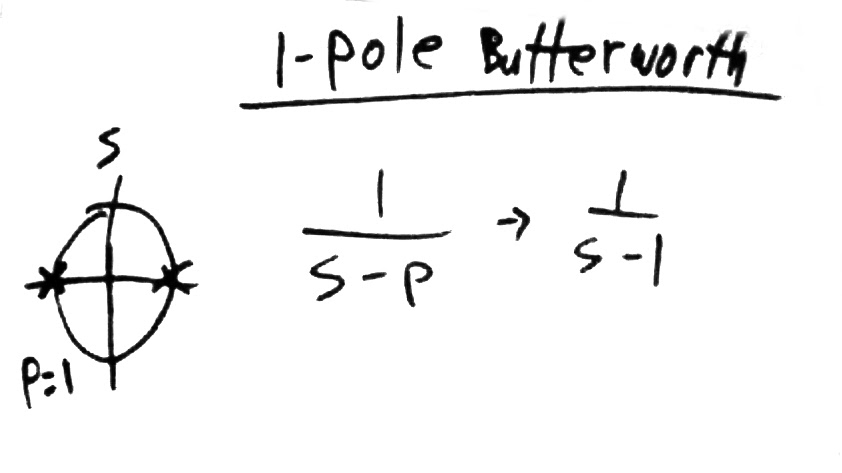
\includegraphics[scale=0.3]{photos/jan26/11f}

This "gives away" the bandwidth of a pole.  
%\subsection*{Frequency scaling}
%
%%\paulhint{See picture taken at 15:48.}
%\paulhint{Another chart taken at 15:49. 11i.jpg}
%
%\subsection*{Finding 3db point}
%
%\paulhint{See pictures at 15:51-2.}
%
%\textbf{Pole bandwidth} = $2 \sigma_p = 2 \pi B$
%
%\subsection*{How to tell if filter is unstable}
%Other ways, without looking at the s-plane and z-plane.
%
%\subsection*{Something}
%\paulhint{See picture at 16:22.}
%
%\subsection*{Something else (laplace transform?)}
%\paulhint{See picture at 16:23.}
%\paulhint{See pictures at 16:25.}
%
%\subsection*{Pole Bandwidth cont.}
%$B =$ bandwidth in Hz\\
%$2 \pi B = 2 \sigma_p$ \\
%
%Let $Z = e^{sT}$
%
%Therefore $Z_p = e^{-pt} = e^{-\sigma_pT} = e^{-\pi B T}$
%
%This is different than the bilinear transform in that it has aliasing. 
%
%$H(s) = \frac{1}{s - p} \leftrightarrow h(t) = e^{pT} =
%e^{-t/\tau}, \sigma_p =-\frac{1}{\tau}$

\subsection*{Complex Resonator}
Move the pole off the DC axis, \\
\paulhint{See pictures at 16:39. 11g}\\
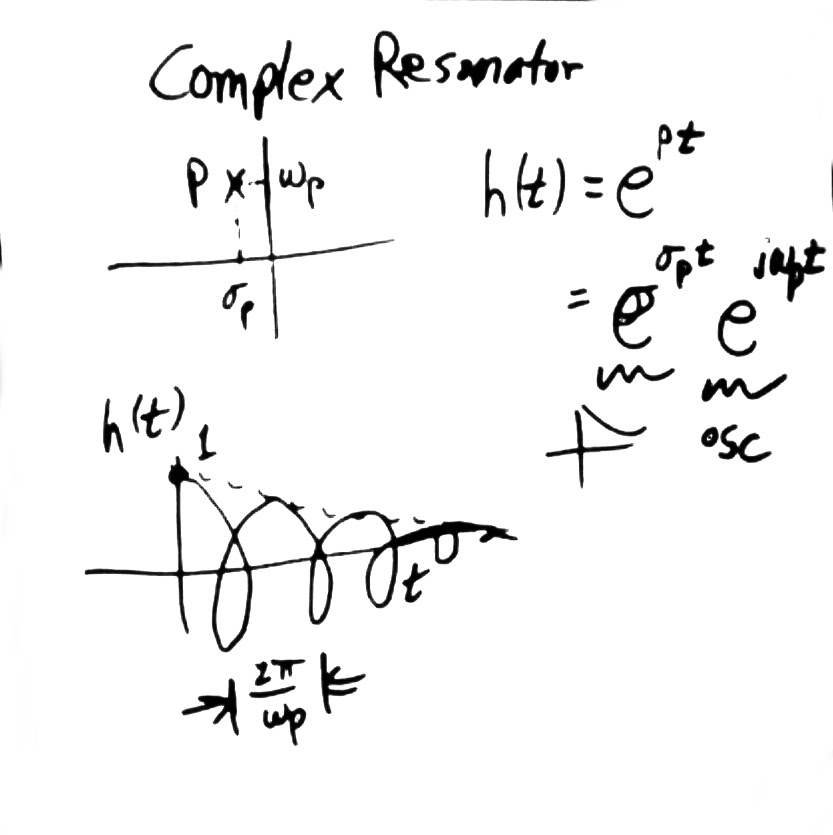
\includegraphics[scale=0.3]{photos/jan26/11g}
%\paulhint{More elaboration at 16:39. 11l}

This is now your basic impulse response resonator. 

Conversion between $t_{60}$ and time constant. It's about a 7th of time constant.
 
